Since the major axis is along the $y$-axis,
\begin{align}
\vec{n} = \vec{e}_2
\end{align}
Thus,
\begin{align}
\vec{V} = \myvec{1&0\\0&1-e^2} \label{eq:chapters/11/11/3/19/5} 
\end{align}
Since
\begin{align}
\vec{c} = \vec{0}, \vec{u}=\vec{0}.
\label{eq:chapters/11/11/3/19/8}
\end{align}
    From \eqref{eq:conic_quad_form},
    \begin{align}
        \vec{P}^\top\vec{VP} + 2\vec{u}^\top\vec{P} + f &= 0 \label{eq:chapters/11/11/3/19/ep1} \\
        \vec{Q}^\top\vec{VQ} + 2\vec{u}^\top\vec{Q} + f &= 0 \label{eq:chapters/11/11/3/19/ep2}
    \end{align}
    yielding
\begin{align}
4e^2 - f = 13 \label{eq:chapters/11/11/3/19/10}
\\
36e^2 - f = 37 \label{eq:chapters/11/11/3/19/11}
\end{align}
which can be formulated as the matrix equation
\begin{align}
\myvec{4&-1\\36&-1}\myvec{e^2\\f} = \myvec{13\\37}
\label{eq:chapters/11/11/3/19/12}
\end{align}
The augmented matrix is given by,
\begin{align}
\myvec{4&-1&\vline&13\\36&-1&\vline&37}
\end{align}
yielding
\begin{align}
\xleftrightarrow[]{R_1\leftarrow R_1-R_2} &\myvec{-32&0&\vline&-24\\36&-1&\vline&37} \\
\xleftrightarrow[]{R_1\leftarrow-\frac{R_1}{8}}& \myvec{4&0&\vline&3\\36&-1&\vline&37} \\
\xleftrightarrow[]{R_2\leftarrow R_2-9R_1}
&\myvec{4&0&\vline&3\\0&-1&\vline&10} \\
\xleftrightarrow[R_2\leftarrow -R_2]{R_1\leftarrow \frac{R_1}{4}}
&\myvec{1&0&\vline&\frac{3}{4}\\0&1&\vline&-10}
\end{align}
Thus,
\begin{align}
e^2 = \frac{3}{4},\ f = -10
\end{align}
and the equation of the conic is given by
\begin{align}
\vec{x}^\top\myvec{1&0\\0&\frac{1}{4}}\vec{x} - 10 = 0
\end{align}
See  
\figref{fig:chapters/11/11/3/19/1}.
\begin{figure}[ht]
\centering
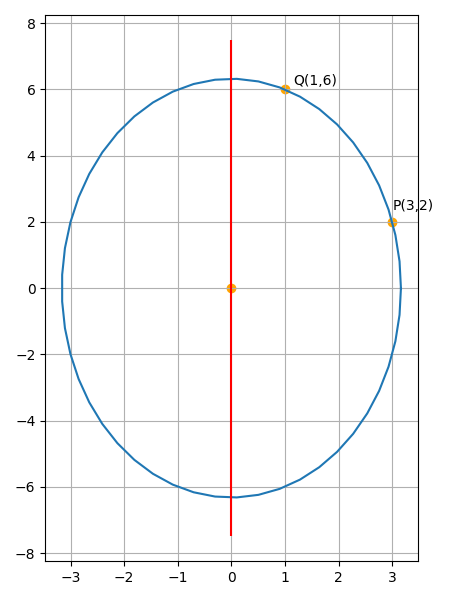
\includegraphics[width = \columnwidth]{chapters/11/11/3/19/figs/fig1.png}
\caption{Graph}
\label{fig:chapters/11/11/3/19/1}
\end{figure}
